\documentclass{article}

% \usepackage[a4paper, margin=1in]{geometry}
\usepackage[preprint]{neurips_2024} % Use this line for submission/drafts
\usepackage[utf8]{inputenc}
\usepackage[T1]{fontenc}
\usepackage{hyperref}
\usepackage{url}
\usepackage{booktabs}       % professional-quality tables
\usepackage{amsfonts}       % blackboard math
\usepackage{nicefrac}       % compact symbols
\usepackage{microtype}      % microtypography
\usepackage{xcolor}         % colors
\usepackage{graphicx}       % for figures
\usepackage{amsmath}        % for math
\usepackage{amssymb}        % for math symbols like \mathbb{R}
\usepackage{tikz}
\usepackage{lscape} % for landscape page
\usepackage{longtable} % for multi-page tables
\usepackage{rotating} 
\usepackage{lmodern}
\usepackage[T1]{fontenc}
\usepackage{textcomp}
\usepackage{colortbl}
\usepackage{subfigure}
\usepackage{subcaption}
\usetikzlibrary{arrows.meta, shapes.geometric, positioning, calc}
\title{Label-Efficient Trajectory Planning in NAVSIM via I-JEPA}

\author{
    Hamza, A., \& Sanchez, A. \\
    Department of Electrical and Computer Engineering \\
    New York University Tandon School of Engineering \\
    \texttt{ah7072@nyu.edu | aas10269@nyu.edux}
}

\begin{document}
\maketitle

\begin{abstract}
 In this study, we explore the integration of Image-based Joint-Embedding Predictive Architecture (I-JEPA) with the NAVSIM Data-Driven Non-Reactive Autonomous Vehicle Simulation framework. I-JEPA, a self-supervised learning paradigm designed to model predictive abstractions without relying on generative pixel-space reconstruction, is particularly well-suited for the structured yet stochastic nature of driving environments. We leverage real-world camera sensor data extracted from the NAVSIM dataset to train the I-JEPA model, capturing the spatiotemporal dependencies inherent in dynamic road scenes. Additionally, the report reviews NAVSIM's benchmark tests performed on the trained I-JEPA model for car trajectory prediction showing that this model is up to par with existing vision-based baselines. This gives the possibility that the I-JEPA model can be improved and thus allow vision tasks to become more "human-like" opening the door for numerous new opportunities. 
\end{abstract}

\section{Introduction}
Autonomous driving systems critically depend on robust perception modules capable of accurately interpreting complex driving environments. As the field of machine learning grows the need for machines to see the world in a more "human-like" view has been a key component in many research endeavors. 
Reliable perception enables autonomous vehicles to identify and respond appropriately to diverse road conditions, environmental changes, and dynamic obstacles, thus significantly enhancing safety, efficiency, and overall operational effectiveness. A decision-making model explored in this paper is Self-supervised learning (SSL), it has emerged as a powerful paradigm for representation learning, eliminating the need for large labeled datasets while achieving competitive performance in downstream tasks. Among SSL approaches, the \textit{Implicit Joint-Embedding Predictive Architecture} (I-JEPA) offers a novel framework that learns by predicting high-level latent representations of missing image regions, rather than reconstructing pixels or enforcing contrastive invariance. This property makes I-JEPA particularly suitable for domains requiring \textit{semantic abstraction}, such as autonomous driving that requires instant decision making in complex scenarios.

However, achieving consistently reliable perception remains challenging, primarily due to the dependence on extensive annotated datasets required by traditional supervised learning approaches. Such datasets are not only expensive and labor-intensive to produce but frequently lack sufficient diversity and variability to adequately train robust models capable of performing effectively across different scenarios and conditions. These limitations have prompted researchers and industry stakeholders alike to explore alternative approaches to perception model training.

In this research, we propose an innovative approach integrating I-JEPA with NAVSIM—a sophisticated, data-driven, non-reactive autonomous vehicle simulation and benchmarking platform designed to replicate realistic driving scenarios. Our method involves leveraging an ImageNet pre-trained I-JEPA Vision Transformer (ViT-B/16) encoder, provided by Meta AI, as a fixed or partially fine-tuned feature extractor and training it using extensive real-world imagery captured by camera sensors from the NAVSIM dataset. This dataset, rich in visual complexity and representative of diverse driving conditions, allows the model to learn nuanced and detailed representations that closely mirror real-world perception challenges. This visual backbone is combined with a lightweight MLP planning head that processes ego-vehicle status and predicts future trajectories. Due to computational resource constraints, we conduct fine-tuning and evaluation on representative subsets of the NAVSIM dataset. 

We propose experiments to evaluate the performance of this I-JEPA-based agent against baselines using NAVSIM's Predictive Driver Model Score (PDMS) and specifically assess its label efficiency by training on varying fractions of the data subset. This work explores the potential of transferring powerful, general-purpose visual representations learned via I-JEPA to the complex, sequential decision-making task of autonomous driving planning, aiming for improved data efficiency.

%By training I-JEPA on these real-world images, our approach effectively captures realistic visual variations, complexities, and intricacies inherent to actual driving environments, thereby significantly enhancing the generalization and adaptability of perception modules. NAVSIM benchmark techniques provide comprehensive tools for systematically evaluating the robustness and performance of these self-supervised representations across various critical perception tasks, including lane marking detection, obstacle classification, pedestrian recognition, and environmental understanding under diverse conditions such as varying lighting, weather, and urban complexity.

%Through rigorous experimental evaluation using NAVSIM benchmarking, we validate the efficacy of our integrated approach. Our findings demonstrate substantial improvements in the accuracy, resilience, and robustness of autonomous vehicle perception modules when employing I-JEPA-trained representations compared to traditional supervised learning methods. Notably, our approach effectively reduces the dependency on annotated data while simultaneously bridging the simulation-to-real-world performance gap.

%Ultimately, this study emphasizes the considerable potential of combining advanced self-supervised learning methodologies, such as I-JEPA, with sophisticated simulation frameworks like NAVSIM. The resulting integration represents a significant advancement towards scalable, robust, and economically viable autonomous driving systems, paving the way for more practical and widespread adoption of autonomous vehicle technologies.
\label{sec:related}

\subsection{Importance of Accurately Predicting a Driving Path}
\label{sec:Importance}

Self-supervised learning methods have emerged as a particularly promising alternative, offering the capability to learn informative representations from unlabeled data by leveraging intrinsic structures within the data itself. Among these, the Image-based Joint-Embedding Predictive Architecture (I-JEPA) stands out as a cutting-edge framework capable of learning robust and generalizable representations through predictive self-supervised objectives. Unlike conventional supervised approaches, I-JEPA does not depend heavily on labeled datasets, enabling more scalable, cost-effective, and flexible training strategies.

Training I-JEPA on these real-world images, our approach effectively captures realistic visual variations, complexities, and intricacies inherent to actual driving environments, thereby significantly enhancing the generalization and adaptability of perception modules. NAVSIM benchmark techniques provide comprehensive tools for systematically evaluating the robustness and performance of these self-supervised representations across various critical perception tasks, including lane marking detection, obstacle classification, pedestrian recognition, and environmental understanding under diverse conditions such as varying lighting, weather, and urban complexity.

\subsection{I-JEPA’s Existing Applications in Driving}

The application of self-supervised learning to autonomous driving has gained momentum, with I-JEPA being recently explored in the context of 3D object detection. A major advancement in this area is AD-L-JEPA \citep{zhu2025adljepa}, which extends I-JEPA to LiDAR-based representation learning. Instead of reconstructing raw point cloud data, AD-L-JEPA predicts embeddings from spatially unknown regions. It improves the quality of the data modeling. What is meant by this is that the embeddings contain relevant details about specific objects in the image that could have been hidden or not captured otherwise. 

Empirical evaluations have shown that AD-L-JEPA outperforms prior self-supervised LiDAR models such as Occupancy-MAE and ALSO, demonstrating superior transferability to 3D object detection tasks. This reinforces the idea that predictive feature-space learning is more effective than pixel-wise reconstruction for autonomous perception \citep{zhu2025adljepa}.

However, no direct application of I-JEPA to camera-based autonomous driving exists. The majority of prior research has focused on contrastive learning (e.g., BYOL, SimCLR, DINO) and generative approaches (MAE, Occupancy-MAE), leaving a gap in the exploration of latent-space predictive learning for end-to-end vision-based driving tasks.

\subsection{I-JEPA: Theoretical Foundations}

\subsubsection{Overview of Joint-Embedding Predictive Architecture (I-JEPA)}
The \textit{Implicit Joint-Embedding Predictive Architecture} (I-JEPA) \citep{assran2023ijepa} is a self-supervised learning framework that learns by predicting high-level latent representations of missing image regions, rather than reconstructing raw pixels. Unlike traditional generative models that require pixel-wise reconstruction, I-JEPA operates in a \textit{feature space}, allowing it to learn more abstract and semantic representations. This is possible by the transformers in the architecture that makes I-JEPA which translates an incoming image into a lower dimensional space keeping the most relevant information of the image. 

I-JEPA follows a \textit{predictive modeling} approach, where the model learns to infer unseen portions of an input image using only its contextual information. This approach is inspired by human perception, where understanding is derived from partial observations rather than complete reconstructions. This characteristic makes I-JEPA particularly effective in learning transferable representations that can generalize across multiple downstream tasks, such as classification, segmentation, and object detection. Thus allowing it to work in many scenarios without depending on the pixels of an image. 

\subsubsection{Core Principles: Context and Target Encoders, Feature Space Prediction}
I-JEPA consists of three primary components:
\begin{itemize}
    \item \textbf{Context Encoder:} Processes a visible portion of the input (referred to as the \textit{context block}) and encodes it into a latent space representation(compressing the image into lower dimension but still keeping it's important features).
    \item \textbf{Target Encoder:} Independently encodes the withheld regions (\textit{target blocks}) into feature representations. Unlike contrastive learning, these target blocks are not augmented variants of the same input but rather different masked-out regions. In other words the Target Encoder takes in the same image that goes into the context encoder, and masks out certain regions of an image. It takes these masked regions and compresses it into a latent space dimension. 
    \item \textbf{Predictor Network:} A lightweight neural network that takes both the context encoding, target encoding and attempts to predict the target encoding in feature space. 
\end{itemize}

I-JEPA does not need to encode the entire input image, and only takes in a section of the image that has not been masked by the target encoder. This allows it to not have to intake numerous unlabeled data, and only a subset. Instead of directly reconstructing pixel-level details, the predictor is trained to minimize the difference between the predicted and actual target embeddings, typically using an $\ell_2$ loss function in the representation space. This design ensures that I-JEPA captures \textit{high-level semantic information} rather than low-level textures, making it more efficient for representation learning.

\subsection{Advantages Over Generative and Contrastive Methods}
I-JEPA differs from existing self-supervised learning approaches in several fundamental ways:

\paragraph{1. No Pixel Reconstruction (vs. Generative Models like MAE)} Masked Autoencoders (MAE) \citep{he2022mae} learn by reconstructing missing pixel values from a heavily masked image. This forces the model to focus on low-level pixel statistics rather than learning abstract, semantic concepts. In contrast, I-JEPA operates in feature space, allowing it to learn more structured and semantically meaningful representations.

\paragraph{2. No Contrastive Loss or Data Augmentations (vs. SimCLR, BYOL)} Contrastive learning methods like SimCLR \citep{chen2020simple} and BYOL \citep{grill2020bootstrap} rely on aggressive data augmentations and instance discrimination. These methods require large batch sizes and careful negative sampling to avoid collapse. I-JEPA, in contrast, does not use negative samples or augmentation-based instance discrimination. 

\paragraph{3. More Efficient and Scalable} Since I-JEPA does not require explicit contrastive negatives or complex generative decoders, it is computationally more efficient. It scales effectively with Vision Transformers (ViTs) and has been shown to perform well even with limited computational resources. 

\subsection{NAVSIM: Theoretical Foundations}
\label{sec:navsim}
\textbf{NAVSIM} \cite{dauner2024navsim} serves as a large-scale, data-driven simulation framework designed specifically for benchmarking autonomous vehicle planning agents. It utilizes real-world sensor recordings from the OpenScene dataset \cite{OpenScene2023}, which provides multimodal data including camera imagery, LiDAR point clouds, and HD map information for a single \emph{ego-vehicle}. The primary task within NAVSIM is trajectory planning: given sensor data history, current ego status, and a high-level driving command, the agent must predict the ego-vehicle's future trajectory as a sequence of $(x, y, \theta)$ poses in its local coordinate frame, typically over a 4-second horizon.

A key characteristic of NAVSIM is its \textbf{non-reactive simulation} approach for evaluation. While the ego-vehicle's predicted trajectory is simulated forward using a kinematic model and controller to check for feasibility and safety, the background traffic agents strictly follow their recorded log trajectories. This design choice ensures deterministic reproducibility and computational efficiency, allowing large-scale evaluation directly on real sensor data without requiring complex reactive agent modeling or synthetic sensor generation.

Evaluation in NAVSIM relies on simulation-based metrics aggregated into the \textbf{Predictive Driver Model Score (PDMS)} \cite{dauner2024navsim, hallgarten2023pdm}. Instead of solely relying on displacement errors relative to the human driver (which can be misleading \cite{zhairet2023rethinking}), PDMS assesses the quality of the planned trajectory by simulating its execution and measuring critical aspects like:
\begin{itemize}
    \item Safety: No-collision (NC) with other agents or static objects (with at-fault logic), Drivable Area Compliance (DAC), Time-to-Collision (TTC).
    \item Comfort: Limits on longitudinal/lateral acceleration and jerk (C).
    \item Progress: Ego Progress (EP) along the intended route compared to a reference planner.
\end{itemize}
These sub-metrics are combined into a single scalar score ($[0, 1]$), providing a holistic assessment of planning performance. The framework also supports filtering mechanisms to remove penalties if the recorded human driver also violated a specific rule (False-Positive Penalty Filtering).

For standardized training and testing, NAVSIM provides curated data splits, \texttt{navtrain} and \texttt{navtest}. These are derived from the full OpenScene dataset but filtered to enrich the proportion of challenging driving scenarios where simple heuristic policies often fail \cite{dauner2024navsim}. For our vision-based agent development, the essential inputs provided by NAVSIM for each scenario timestep include:
\begin{enumerate}
    \item The front camera image (\texttt{cam\_f0}).
    \item Past ego motion history (velocity and acceleration).
    \item A discrete driving command (e.g., left, straight, right) derived from the planned route.
\end{enumerate}

\begin{figure}[ht]
    \centering
    % Resize the whole picture to fit the line width
    \resizebox{\linewidth}{!}{% Add this line
    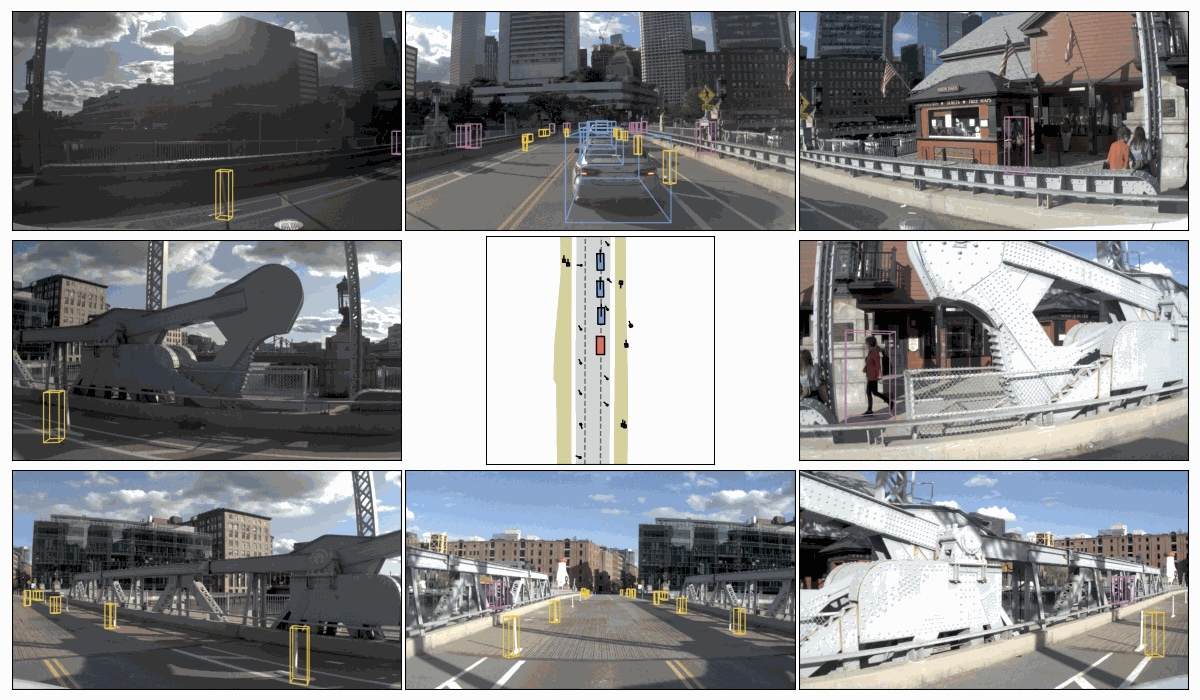
\includegraphics[width=0.8\linewidth]{images/data-sample-1.jpg}
    \hfill
    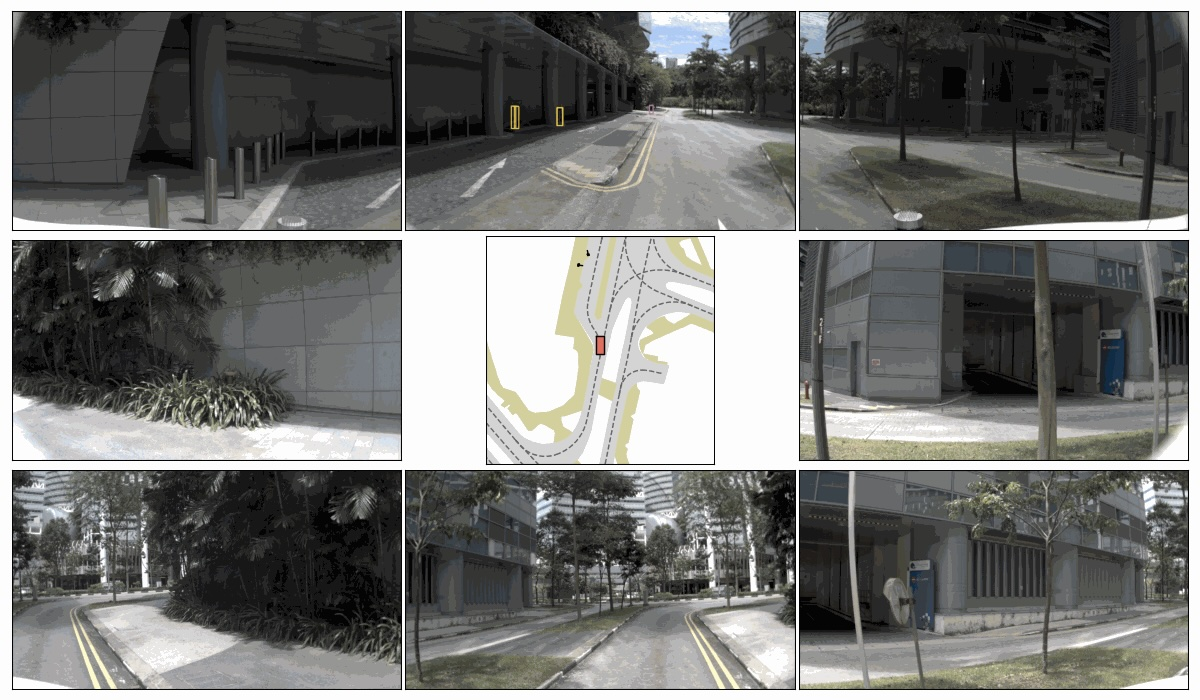
\includegraphics[width=0.8\linewidth]{images/data-sample-2.jpg}
    }
    \caption{NAVSIM frames of various cameras and sensors}
    \label{fig:navsim_scenario}
\end{figure}

While other sensor data like LiDAR is available, our approach focuses primarily on leveraging the visual input via the I-JEPA encoder as shown in Figure~\ref{fig:navsim_scenario}. 

\textbf{PDM Score}
The Predictive Driver Model Score (PDMS) evaluates planned trajectories by aggregating key safety, legality, and comfort aspects into a single scalar. It is defined as:

\begin{equation}
    \text{PDMS} = \left( \prod_{m \in \{\text{NC}, \text{DAC}\}} \text{score}_m \right) \times \left( \frac{\sum_{w \in \{\text{EP}, \text{TTC}, \text{C}\}} \text{weight}_w \times \text{score}_w}{\sum_{w \in \{\text{EP}, \text{TTC}, \text{C}\}} \text{weight}_w} \right)
    \label{eq:pdms}
\end{equation}

where penalties (NC, DAC) are multiplicative, and rewards (EP, TTC, C) are aggregated with weighted averaging.

\textbf{No-At-Fault Collisions (NC)}
Measures whether the ego-vehicle avoids collisions it would be responsible for.
\begin{equation}
    \text{score}_{\text{NC}} = 
    \begin{cases}
        1, & \text{no collision} \\
        0.5, & \text{collision with static object} \\
        0, & \text{collision with dynamic agent}
    \end{cases}
\end{equation}

\textbf{Drivable Area Compliance (DAC)}
Checks if all corners of the ego-vehicle remain within drivable regions (lanes, intersections, parking areas).
\begin{equation}
    \text{score}_{\text{DAC}} =
    \begin{cases}
        1, & \text{all trajectory points inside drivable area} \\
        0, & \text{any point outside}
    \end{cases}
\end{equation}

\textbf{Ego Progress (EP)}
Evaluates how much progress the ego-vehicle makes compared to an expert planner's safe upper bound.
\begin{equation}
    \text{score}_{\text{EP}} = \min\left( 1, \frac{\text{progress}_{\text{ego}}}{\text{progress}_{\text{expert}}} \right)
\end{equation}

\textbf{Time-to-Collision Compliance (TTC)}
Assesses if a safe time-to-collision margin is maintained throughout the trajectory.
\begin{equation}
    \text{score}_{\text{TTC}} =
    \begin{cases}
        1, & \text{TTC} > 0.9 \, \text{seconds} \quad \forall t \\
        0, & \text{otherwise}
    \end{cases}
\end{equation}

\textbf{Comfort (C)}
Ensures smoothness by enforcing bounds on longitudinal acceleration, lateral acceleration, and jerk.
\begin{equation}
    \text{score}_{\text{C}} =
    \begin{cases}
        1, & \text{all acceleration and jerk thresholds satisfied} \\
        0, & \text{otherwise}
    \end{cases}
\end{equation}

\textbf{Driving Direction Compliance (DDC)}
(Collected but not counted in PDMS.) Verifies that driving remains aligned with allowed road directions.

\textbf{Traffic Light Compliance (TLC)}
(Collected but not counted in PDMS.) Checks if traffic lights at crossings are respected.

\textbf{Lane Keeping (LK)}
(Additional metric, not core to PDMS.) Measures if the ego-vehicle remains centered within its designated lane.

\subsubsection{Dataset}
The  chosen OpenScene \cite{OpenScene2023}, a redistribution of nuPlan \cite{karnchanachari2024nuplan}, the largest annotated public driving dataset. OpenScene
includes 120 hours of driving at a reduced frequency of 2Hz typically considered by end-to-end
planning algorithms, resulting in a 90\% reduction of data storage requirements compared to nuPlan
from over 20 TB to 2 TB. Our agent input, based on OpenScene, comprises of one front view camera, with a resolution of 1920 × 1080 pixels. The input
includes the current time-step and optionally 3 past frames, totaling 1.5s at 2Hz.\cite{dauner2024navsim}

\section{Methodology}
% Slide 6: Methodology: Pipeline
\begin{figure}[ht]
    \centering
    % Resize the whole picture to fit the line width
    \resizebox{\linewidth}{!}{% Add this line
    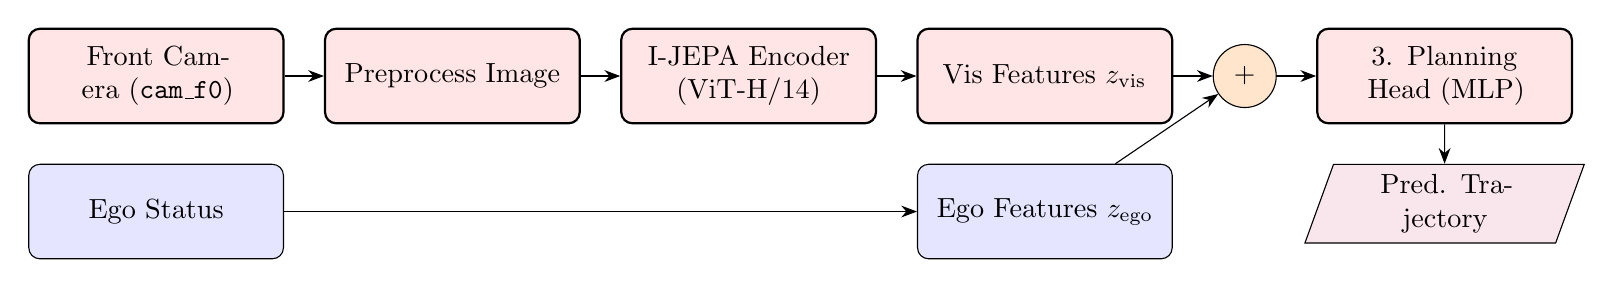
\begin{tikzpicture}[
        node distance=1cm and 1.5cm, % Keep original distances for now
        block/.style={rectangle, draw, fill=blue!10, rounded corners,
                      text width=3cm, text centered, minimum height=1.2cm},
        data/.style={ellipse, draw, fill=green!10, text centered, minimum width=2cm},
        arrow/.style={-{Stealth[length=2mm, width=1.5mm]}},
        concat/.style={circle, draw, fill=orange!20, minimum size=0.8cm, inner sep=0pt, node contents={+}},
        module/.style={rectangle, draw, fill=red!10, rounded corners, thick,
                       text width=3cm, text centered, minimum height=1.2cm},
        output/.style={trapezium, trapezium left angle=70, trapezium right angle=110, draw, fill=purple!10,
                       text width=2.5cm, text centered, minimum height=1cm},
        comment/.style={rectangle, text width=4cm, align=left, font=\small\itshape}
      ]

      % --- Original TikZ Nodes and Arrows ---
      % Input Data Nodes
      % \node (navsim) [block, fill=gray!10] {NAVSIM};
      \node (cam_img) [module] {Front Camera (\texttt{cam\_f0})}; % Shortened text
      \node (ego_status) [block, below=0.5cm of cam_img] {Ego Status}; % Shortened text
      % Processing Steps
      \node (preprocess) [module, right=0.5cm  of cam_img] {Preprocess Image}; % Shortened text
      \node (encoder) [module, right=0.5cm  of preprocess] {I-JEPA Encoder (ViT-H/14)}; % Shortened text
      \node (vis_feat) [module, right=0.5cm  of encoder] {Vis Features $z_{\text{vis}}$}; % Shortened text
      \node (ego_feat) [block, below=0.5cm  of vis_feat] {Ego Features $z_{\text{ego}}$};

      % % Fusion and Planning Head
      \node (concatenate) [concat, right=0.5cm of vis_feat] {};
      \node (head) [module, right=0.5cm of concatenate] {3. Planning Head (MLP)};
      \node (traj_pred) [output, below=0.5cm of head] {Pred. Trajectory}; % Shortened text

      % % Arrows indicating data flow
      \draw [arrow] (cam_img) -- (preprocess);
      \draw [arrow] (preprocess) -- (encoder);
      \draw [arrow] (encoder) -- (vis_feat);
      \draw [arrow] (ego_status) -- (ego_feat);
      \draw [arrow] (vis_feat) -- (concatenate);
      \draw [arrow] (ego_feat) -- (concatenate);
      \draw [arrow] (concatenate) -- (head);
      \draw [arrow] (head) -- (traj_pred);

    \end{tikzpicture}
    } % Add this closing brace for resizebox
    \caption{Pipeline for the I-JEPA-based planning agent in NAVSIM.} % Shortened caption
    \label{fig:pipeline}
\end{figure}
\subsection{Pre-trained I-JEPA Encoder}
\label{subsec:encoder}
% State the chosen approach directly and justify it.
Our approach leverages a publicly available, pre-trained I-JEPA model to serve as the visual encoder for our NAVSIM planning agent. This strategy allows us to utilize powerful, general-purpose visual features learned on large-scale datasets (ImageNet-1K) without undertaking the computationally intensive self-supervised pre-training process ourselves. We specifically adopt the official \textbf{ViT-H/14} I-JEPA checkpoint released by Meta AI \cite{assran2023ijepa}.

% Specify which parts are used and discarded.
From the complete I-JEPA architecture associated with the checkpoint, we isolate and utilize only the \textbf{context encoder} component ($f_\theta$). The target encoder ($f_{\bar{\theta}}$) and the predictor network ($g_\phi$), which are essential for the I-JEPA pre-training objective, are discarded for our downstream planning task.

% Detail the integration process: how the encoder processes NAVSIM input.
The selected ViT-H/14 context encoder has specific input requirements. To integrate it into our NAVSIM agent, the following processing pipeline is applied at each timestep the agent needs to make a prediction:
\begin{enumerate}
    % Step 1: Input Extraction - Explicitly mention the source camera.
    \item The image from the ego-vehicle's primary front camera (\texttt{cam\_f0}) is obtained from the current NAVSIM scenario data \cite{dauner2024navsim, OpenScene2023}.
    % Step 3: Normalization - Crucial for pre-trained models.
    \item The image tensor is then passed through the loaded ViT-H/14 context encoder ($f_\theta$).
    % Step 5: Feature Extraction - Specify the exact feature used.
    \item The final visual feature representation for the planning head is obtained by extracting the output embedding corresponding to the special \texttt{[CLS]} token \cite{dosovitskiy2020vit}. For the ViT-H/14 architecture, this results in a feature vector $z_{\text{vis}} \in \mathbb{R}^{768}$.
\end{enumerate}

% Describe how the encoder's weights are handled during downstream fine-tuning.
During the subsequent fine-tuning phase on the NAVSIM trajectory prediction task (detailed in Sec.~\ref{subsec:subset}), the parameters of this pre-trained encoder are managed according to one of two strategies:
\begin{itemize}
    \item \textbf{Stage 1 (Frozen Encoder):} Initially, all parameters of the loaded ViT-B/16 encoder are frozen (i.e., their gradients are not computed or updated). Training only affects the parameters of the planning head (Sec.~\ref{subsec:head}). This stage evaluates the direct utility of the off-the-shelf ImageNet-trained I-JEPA features for the driving task.
    \item \textbf{Stage 2 (Partial Fine-tuning, Optional):} After an initial training period with the encoder frozen, we may selectively unfreeze the parameters of the final transformer block(s) and associated layer normalization layers within the ViT encoder. These layers, along with the planning head, are then trained jointly, typically employing a much smaller learning rate for the encoder parameters ($\alpha_{\text{enc}}$) compared to the head ($\alpha_{\text{head}}$) (e.g., $\alpha_{\text{enc}} = \alpha_{\text{head}} / 10$). This allows the higher-level features of the encoder to adapt slightly to the specific visual characteristics of the NAVSIM environment while aiming to preserve the robust representations learned during pre-training.
\end{itemize}

% \subsection{Planning Head}
% \label{subsec:head}
% We employ a simple Multi-Layer Perceptron (MLP) as the planning head. This head takes the concatenated visual features and ego status information as input and predicts the future trajectory.
% \begin{itemize}
%     \item \textbf{Input Features:} The input to the MLP is the concatenation of the visual feature $z_{\text{vis}} \in \mathbb{R}^{768}$ (from the I-JEPA encoder's \texttt{[CLS]} token) and the current ego status features $z_{\text{ego}} \in \mathbb{R}^{7}$. The ego status features consist of 2D velocity, 2D acceleration, and a 3-dimensional one-hot encoding of the driving command (left, right, straight), resulting in a combined input dimension of $768 + 7 = 775$.
%     \item \textbf{Architecture:} The MLP consists of two hidden layers, each with 256 neurons and ReLU activation functions.
%     \item \textbf{Output:} The final linear layer maps the 256-dimensional hidden representation to the flattened trajectory parameters. For a 4-second horizon sampled at 0.5-second intervals ($N_{\text{poses}} = 8$), the output dimension is $N_{\text{poses}} \times 3 = 8 \times 3 = 24$. This output is then reshaped into the trajectory format $[N_{\text{poses}}, 3]$, where each row represents $(x, y, \theta)$ in the local ego-vehicle coordinate frame at future timesteps $\{0.5, 1.0, \dots, 4.0\}\,\text{s}$.
%     \item \textbf{Training Loss:} The planning head (and optionally the unfrozen encoder layers) is trained using an $L_1$ loss between the predicted trajectory and the ground-truth future trajectory recorded by the human driver in the NAVSIM logs.
% \end{itemize}

% \subsection{Planning Head}
% \label{subsec:head}
% The planning head serves as the crucial component that maps the rich features extracted by the visual encoder and the current vehicle state into a concrete future trajectory plan. For this initial investigation, we employ a relatively simple \textbf{Multi-Layer Perceptron (MLP)} architecture for this head.

% % Justification for choosing MLP
% The choice of an MLP is deliberate, driven by several factors:
% \begin{itemize}
%     \item \textbf{Simplicity and Efficiency:} MLPs are straightforward to implement, computationally efficient to train and run, and provide a solid baseline for regression tasks.
%     \item \textbf{Focus on Features:} By using a simple head, we aim to primarily evaluate the quality and utility of the semantic features ($z_{\text{vis}}$) derived from the pre-trained I-JEPA encoder. A more complex head (e.g., a Transformer decoder) might achieve higher performance but could also obscure whether improvements stem from the head's architecture or the input features themselves.
%     \item \textbf{Baseline Establishment:} It establishes a performance benchmark. If strong results can be achieved even with this simple head, it strongly suggests the high quality of the I-JEPA features for this task. Future work could then explore more complex head architectures.
% \end{itemize}

% % Detailed Structure Description
% The specific structure of our MLP planning head is as follows:
% \begin{itemize}
%     \item \textbf{Input Features:} The input layer receives the concatenated feature vector, combining the visual embedding $z_{\text{vis}} \in \mathbb{R}^{768}$ (from the I-JEPA encoder's \texttt{[CLS]} token, Sec.~\ref{subsec:encoder}) and the current ego status features $z_{\text{ego}} \in \mathbb{R}^{7}$ (2D velocity, 2D acceleration, and a 3-dimensional one-hot encoding for the driving command: left, right, or straight). This results in a combined input vector of dimension $768 + 7 = 775$.
%     \item \textbf{Hidden Layers:} The MLP incorporates two hidden layers.
%         \begin{itemize}
%             \item The first hidden layer performs a linear transformation from the 775-dimensional input to 256 neurons, followed by a Rectified Linear Unit (ReLU) activation function. ReLU is chosen for its computational efficiency and ability to introduce non-linearity, allowing the network to model complex relationships.
%             \item The second hidden layer applies another linear transformation from 256 neurons to 256 neurons, again followed by a ReLU activation.
%         \end{itemize}
%     \item \textbf{Output Layer:} A final linear layer maps the 256-dimensional representation from the last hidden layer to the required output dimension for the trajectory. For the standard NAVSIM 4-second planning horizon sampled at 0.5-second intervals ($N_{\text{poses}} = 8$), the output consists of 8 poses, each with $(x, y, \theta)$ coordinates. Therefore, the output layer has $N_{\text{poses}} \times 3 = 8 \times 3 = 24$ neurons. This layer uses \textit{no activation function}, as is standard for regression tasks where the output values are unbounded (or bounded by subsequent processing/interpretation rather than the activation itself).
%     \item \textbf{Output Reshaping:} The flattened 24-dimensional output vector is then reshaped into the standard trajectory format $[N_{\text{poses}}, 3]$ (i.e., $[8, 3]$), where each row represents the predicted $(x, y, \theta)$ pose in the local ego-vehicle coordinate frame at future timesteps $\{0.5, 1.0, \dots, 4.0\}\,\text{s}$.
% \end{itemize}

\subsection{Planning Head}
\label{subsec:head}
The planning head serves as the crucial component that maps the features extracted by the visual encoder and the ego vehicle's state into a concrete future trajectory plan. For this study, we primarily employ a \textbf{Multi-Layer Perceptron (MLP)} architecture for this head.

The choice of an MLP is deliberate, driven by factors such as simplicity, computational efficiency, and its suitability for establishing a performance baseline to evaluate the quality of input features (visual and ego state).

\paragraph{Initial MLP Architecture (Experiments 1-3):}
Our initial baseline MLP architecture, used in Experiments 1 through 3, had the following structure:
\begin{itemize}
    \item \textbf{Input Features:} The input layer received a concatenated feature vector.
        \begin{itemize}
            \item Visual embedding $z_{\text{vis}} \in \mathbb{R}^{1280}$: Obtained from the I-JEPA encoder's output (using Pooler Output or Mean Pooling, based on configuration). Note that the ViT-H/14 model used provides features of this dimension, differing from the ViT-B/16 mentioned in the initial problem statement.
            \item Current ego status features $z_{\text{ego}} \in \mathbb{R}^{8}$: Consisting of 2D velocity, 2D acceleration, and a 4-dimensional one-hot encoding for the driving command (matching the data format).
        \end{itemize}
    This resulted in an initial combined input vector dimension of $1280 + 8 = 1288$.
    \item \textbf{Hidden Layers:} This MLP incorporated \textbf{three} hidden layers.
        \begin{itemize}
            \item Each hidden layer performed a linear transformation followed by a Rectified Linear Unit (ReLU) activation and a Layer Normalization.
            \item All hidden layers used 256 neurons.
        \end{itemize}
    \item \textbf{Output Layer:} A final linear layer mapped the 256-dimensional representation from the last hidden layer to the required output dimension for the trajectory ($N_{\text{poses}} \times 3$). For the standard NAVSIM 4-second horizon sampled at 0.5-second intervals ($N_{\text{poses}} = 8$), the output layer had $8 \times 3 = 24$ neurons and used no activation function.
    \item \textbf{Output Reshaping:} The flattened 24-dimensional output vector was reshaped into the standard trajectory format $[8, 3]$.
\end{itemize}
This baseline MLP had approximately 469k trainable parameters.

\paragraph{Incorporating Ego History (Experiments 4-6):}
To better capture the vehicle's motion dynamics, we modified the input features to include historical ego status.
\begin{itemize}
    \item Instead of just the current ego status ($\mathbb{R}^{8}$), the \textbf{last $N=4$ frames} of ego status (velocity, acceleration, command) were extracted.
    \item The 8-dimensional feature vectors for each of these 4 historical frames were \textbf{concatenated} into a single larger ego feature vector.
    \item This resulted in an expanded ego status input dimension of $4 \times 8 = 32$.
\end{itemize}
The input layer of the MLP was adapted to accept this new, larger concatenated input vector. The combined input dimension for Experiments 4 through 6 became $1280$ (Visual) + $32$ (Ego History) = \textbf{1312}. The number of trainable parameters for the MLP with 3 hidden layers slightly increased to $\sim$475k due to the larger input layer.

\paragraph{MLP Architecture Upgrade (Experiment 6):}
In Experiment 6, we further explored increasing the capacity of the MLP planning head.
\begin{itemize}
    \item We added \textbf{one additional hidden layer} to the MLP.
    \item The structure became: Input $\rightarrow$ H $\rightarrow$ H $\rightarrow$ H $\rightarrow$ H $\rightarrow$ Output (4 hidden layers).
    \item Each hidden layer retained 256 neurons, with ReLU and Layer Normalization.
    \item This architecture was used with the 4-frame ego history input.
\end{itemize}
This upgraded MLP with 4 hidden layers and 4-frame ego history had approximately 541k trainable parameters.

\paragraph{Training Loss:}
The parameters of the trainable planning head (and potentially the unfrozen encoder layers during Stage 2 fine-tuning) are optimized by minimizing the difference between the model's predicted trajectory and the ground-truth future trajectory. We employ the \textbf{L1 loss} (Mean Absolute Error) for this task. Specifically, the L1 loss is computed between the model's predicted trajectory (converted to absolute coordinates using the ground-truth current ego pose) and the absolute ground-truth future trajectory recorded in the NAVSIM logs.

L1 loss was selected over alternatives like L2 loss (Mean Squared Error) due to its desirable properties for trajectory regression:
\begin{itemize}
    \item \textbf{Robustness to Outliers:} L1 loss is less sensitive to large errors or anomalies present in human-recorded ground truth trajectories compared to L2 loss, which squares the errors, giving disproportionate weight to large deviations.
    \item \textbf{Direct Interpretation:} L1 loss provides a straightforward and interpretable measure of the average absolute error for each predicted coordinate (lateral offset, longitudinal distance, and heading) across all predicted poses in the trajectory.
    \item \textbf{Common Practice:} L1 loss is a frequently adopted objective function within the trajectory prediction and motion planning literature, facilitating comparison with existing work and baselines.
\end{itemize}

\subsection{Fine-tuning on NAVSIM Subsets}
\label{subsec:subset}
The standard training configuration within the NAVSIM framework utilizes the \texttt{navtrain} split \cite{dauner2024navsim}. This split is itself a curated filter applied to the large OpenScene \texttt{trainval} dataset logs, specifically selecting over 100,000 challenging driving scenarios where simple heuristic policies often fail. While NAVSIM offers optimized sensor data downloads for \texttt{navtrain} (approx. 445GB), processing even this curated split for numerous experiments can be demanding under the NYU HPC quota limitations and time constraints.

Therefore, to ensure feasible training times and resource usage, our fine-tuning experiments are conducted on a further \textbf{randomly selected subset} derived from the official \texttt{navtrain} split. We define a fixed subset fraction, specifically \textbf{10\%} (corresponding to \(\approx\) 4800 scenarios), sampled once based on scenario tokens. This fixed training subset is used consistently across all experiments, including the training of baseline models (Sec.~\ref{sec:experiments}) and the label efficiency analysis, ensuring fair comparisons.

From this selected training subset, a small portion (e.g., 10\%) is held out to form a distinct \textbf{validation subset}. This validation set is used exclusively for monitoring training progress (e.g., validation loss) and potentially for early stopping, preventing overfitting to the training subset. The NAVSIM \texttt{Dataset} class and data loading scripts are configured to load only the scenario tokens corresponding to our defined training and validation subsets.

The fine-tuning process will make use the AdamW optimizer \cite{loshchilov2017decoupled} with default hyperparameters, except for the learning rate. We train for a maximum of 50 epochs, using the validation subset loss for potential early stopping. A base learning rate, $\alpha_{\text{head}}$, is applied to the parameters of the planning head (Sec.~\ref{subsec:head}). 

% For the Stage 2 partial fine-tuning (Sec.~\ref{subsec:encoder}), the learning rate for the unfrozen encoder parameters, $\alpha_{\text{enc}}$, is reduced, $\alpha_{\text{enc}} = \alpha_{\text{head}} / 10$. To gauge the robustness of our findings concerning the chosen subset and training stochasticity, key experiments may be repeated using multiple random seeds for the initial subset sampling and model weight initialization.

\subsection{Overview of I-JEPA Agent Model in NAVSIM Environment}
Our I-JEPA model created follows NAVSIM's \texttt{AbstractAgent} as a parent structure. The following classes and functions were included in our agent.

\texttt{class CameraImageFeatureBuilder}
\begin{itemize}
    \item \textbf{Role:} A NAVSIM \texttt{AbstractFeatureBuilder} for camera data.
    \item \textbf{\texttt{compute\_features}}: Extracts the most recent front camera image (\texttt{cam\_f0}) from the \texttt{AgentInput} and returns it as a processed tensor (Channels-Height-Width, float).
\end{itemize}

\texttt{class EgoFeatureBuilder}
\begin{itemize}
    \item \textbf{Role:} A NAVSIM \texttt{AbstractFeatureBuilder} for ego state data.
    \item \textbf{\texttt{compute\_features}}: Extracts and formats the ego vehicle's velocity, acceleration, and driving command (as a one-hot vector) into a single tensor representing the ego state features.
\end{itemize}

\texttt{class TrajectoryTargetBuilderGT}
\begin{itemize}
    \item \textbf{Role:} A NAVSIM \texttt{AbstractTargetBuilder} for ground truth trajectory.
    \item \textbf{\texttt{compute\_targets}}: Retrieves the ground truth future trajectory for the ego vehicle from the \texttt{Scene} object and returns it as a sequence of \emph{absolute} 3D poses (x, y, heading).
\end{itemize}

\texttt{class IJEPAPlanningAgent}
\begin{itemize}
    \item \textbf{Role:} The main planning agent, inheriting from NAVSIM's \texttt{AbstractAgent}.
    \item \textbf{\texttt{initialize()}}: Sets up the agent by loading the pre-trained I-JEPA model (and \emph{freezing} its weights), loading the required processing object (\texttt{AutoProcessor}), and initializing the trainable MLP prediction head. Handles loading pre-trained MLP weights if specified.
    \item \textbf{\texttt{get\_sensor\_config()}}: Declares the specific sensors required by the agent (primarily \texttt{cam\_f0}).
    \item \textbf{\texttt{get\_feature\_builders()}} and \textbf{\texttt{get\_target\_builders()}}: Specifies which feature and target builders the NAVSIM framework should use to prepare the data for the agent.
    \item \textbf{\texttt{forward(features)}}: Implements the prediction pipeline. It processes the image through the frozen I-JEPA encoder, combines the visual features with the ego state features, and passes the result through the trainable MLP to predict a future trajectory (as \emph{relative} poses).
    \item \textbf{\texttt{compute\_loss(features, targets, predictions)}}: Calculates the training loss. It converts the agent's \emph{relative} trajectory predictions to \emph{absolute} coordinates (using the ground truth current pose) and computes the L1 or MSE loss against the absolute ground truth trajectory. Only updates the MLP parameters.
    \item \textbf{\texttt{get\_optimizers()}}: Defines the optimization setup for training. It configures the \texttt{AdamW} optimizer for the trainable MLP parameters and adds a \texttt{CosineAnnealingLR} learning rate scheduler.

\end{itemize}

\vspace{1em} % Add some vertical space before the summary
In summary, the agent leverages feature and target builders to prepare input data and ground truth. The \texttt{initialize} method sets up the frozen visual encoder and the trainable planning MLP. The \texttt{forward} pass combines encoded visual features and ego state to predict a relative trajectory, and \texttt{compute\_loss} evaluates this prediction against the absolute ground truth, optimizing the MLP via the \texttt{get\_optimizers} setup.

% Requires: \usepackage{colortbl}

\section{Experiments}
\label{sec:experiments}
All experiments were conducted on a 10\% subset of the NAVSIM \texttt{navtrain} split, with a fixed 10\% validation split, using a batch size of 32 and the AdamW optimizer. The I-JEPA ViT-H/14 encoder was kept frozen throughout training. Evaluations were performed on a \(\sim\text{1k}\) scenario subset of the \texttt{navtest} split, calculating the PDMS and its sub-metrics. Code changes were made to the custom agent and feature builders to incorporate ego history and modify the MLP architecture. The training process utilized the NAVSIM PyTorch Lightning training module.
\subsubsection*{Experiment 1: Baseline (30 Epochs, No Scheduler)}
This experiment serves as the initial baseline for comparison. The agent used the original MLP architecture (3 hidden layers, 256d, $\sim$469k trainable parameters) and was trained for 30 epochs with a fixed learning rate of 1e-4 and no scheduler. It achieved a test PDMS of 0.8129. The training loss converged to 0.4 and validation loss also remained at 0.4, potentially indicating underfitting or insufficient training time.
\subsubsection*{Experiment 2: Longer Training (50 Epochs, No Scheduler)}
Extending the training duration to 50 epochs with the same architecture and hyperparameters led to a significant improvement in performance. The training loss dropped to 0.211 and validation loss to 0.278, indicating better fitting. The test PDMS increased substantially to \textbf{0.8466}. This run serves as the primary comparison point for subsequent experiments, demonstrating the value of longer training for this initial setup.
\subsubsection*{Experiment 3: Cosine Scheduler (100 Epochs, No History)}
This experiment investigated the impact of a learning rate scheduler. The agent (original MLP, no history) was trained for 100 epochs using a Cosine Annealing LR scheduler (decaying from 1e-4). Training loss continued to decrease (0.160), and validation loss remained stable (0.279). However, the test PDMS slightly decreased to 0.8417 compared to the 50-epoch run without a scheduler. This suggests that while the scheduler helps reduce training loss, it did not translate to better generalization on the PDMS metric beyond 50 epochs for this configuration. Performance on some sub-metrics like EP (0.9132) and LK (0.970) saw slight improvements compared to Exp 2, but overall PDMS was lower.
\subsubsection*{Experiment 4: 4-Frame Ego History (75 Epochs, Cosine)}
Here, we introduced 4 frames of simple concatenated ego history. This increased the MLP trainable parameters slightly to $\sim$475k due to the larger input layer. The agent was trained for 75 epochs with the Cosine scheduler. This experiment showed a relatively high training loss (0.225) and validation loss (0.280) at 75 epochs compared to Exp 2 and 3. The test PDMS was 0.8399, slightly lower than previous bests. While the overall score decreased, some key metrics improved compared to Exp 2: TTC (0.979 vs 0.978) and LK (0.960 vs 0.952). EP (0.9009) slightly decreased compared to Exp 2 (0.9089) but was higher than Exp 1. The higher training loss suggested potential issues with this specific run's convergence.
\subsubsection*{Experiment 5: Resume Training & Lower LR (Total 100 Epochs, 4-Frame History)}
This experiment resumed training from the 75-epoch checkpoint of Exp 4, continuing for 25 more epochs (total 100) with a reduced learning rate of 5e-5 for the resumed portion. This led to a lower final training loss (0.176) and a new best validation loss (0.273) for the configurations with history. The test PDMS increased to 0.8441, recovering some performance lost in Exp 4 but still slightly below the peak of Exp 2. However, it achieved the highest EP (0.9096) and TTC (0.980) scores among all runs, and also the highest LK (0.962). This run represents the best performance achieved *with* 4-frame ego history, indicating that history helps with dynamic metrics when trained appropriately with a lower final learning rate.
\subsubsection*{Experiment 6: Larger MLP (4 Hidden Layers, 125 Epochs)}
In this experiment, we upgraded the MLP architecture to include 4 hidden layers (256d each), increasing trainable parameters to $\sim$541k. The agent with 4-frame ego history was trained for 125 epochs with the Cosine scheduler, starting with LR 5e-5. This configuration resulted in significantly worse performance across the board: higher training loss (0.271), validation loss (0.309), and a much lower PDMS (0.8113). While TTC slightly increased (0.982), other dynamic metrics (EP, LK) and overall score regressed significantly, and the Comfort score (0.818) was unusually low. This suggests that simply increasing the MLP depth/size without further hyperparameter tuning or more data was detrimental. The larger model might have struggled to converge or overfit differently.


\section{Results}
\label{sec:results}

\begin{table}[h]
    \centering
    \setlength{\tabcolsep}{4pt}
    \begin{tabular}{@{}l l l l l l l l@{}}
        \toprule
        \textbf{Exp} & \textbf{Epochs} & \textbf{Main Change} & \textbf{T. Params} & \textbf{Train Loss} ↓ & \textbf{Val Loss} ↓ & \textbf{PDMS} ↑ \\
        \midrule
        1 &  30 & Baseline & 469k & 0.400  & 0.400 & 0.8129 \\
        \midrule
        2 & 50 & Longer training & 469k & 0.211 & 0.278 & \textbf{0.8466} \\
        3 & 100 & Cos Sched.  & 469k & \textbf{0.160} & 0.279 & 0.8417 \\
        \midrule
        4 & 75 & 4-frame ego hist. & 475k & 0.225 & 0.280 & 0.8399 \\
        5 & 100 & Longer training & 475k & 0.176 & \textbf{0.273} & 0.8441 \\
        6 & 125 & Upgraded MLP & 541k & 0.271 & 0.309 & 0.8113 \\
        \bottomrule\\
    \end{tabular}
    \caption{Summary of experimental modifications and their impact on training, validation loss, and PDMS.}
    \label{tab:experiment_summary}
\end{table}


\begin{table}[h]
    \centering
    \begin{tabular}{@{}l l l l l l l l l l@{}}
        \toprule
        \textbf{Exp} & \textbf{PDMS} & \textbf{DDC} & \textbf{TLC} & \textbf{LK} & \textbf{NC} & \textbf{DAC} & \textbf{EP} & \textbf{C} & \textbf{TTC} \\
        \midrule
        1 & 0.8129 & 0.9925 & 0.996 & 0.938 & 0.9665 & 0.952 & 0.8851 & 0.932 & 0.955 \\
        2 & \textbf{0.8466} & \textbf{0.9940} & \textbf{0.997} & 0.952 & \textbf{0.9790} & \textbf{0.954} & 0.9089 & 0.994 & 0.978 \\
        3 & 0.8417 & \textbf{0.9940} & \textbf{0.997} & \textbf{0.970} & \textbf{0.9790} & 0.949 & \textbf{0.9132} & \textbf{0.995} & 0.972 \\
        4 & 0.8399 & \textbf{0.9940} & \textbf{0.997} & 0.960 & 0.9765 & 0.949 & 0.9009 & \textbf{0.995} & 0.979 \\
        5 & 0.8441 & 0.9930 & 0.996 & 0.962 & 0.9770 & 0.950 & 0.9096 & \textbf{0.995} & 0.980 \\
        6 & 0.8113 & 0.9935 & 0.995 & 0.950 & 0.9770 & 0.952 & 0.8872 & 0.818 & \textbf{0.982} \\
        \bottomrule\\
    \end{tabular}
    \caption{PDMS and subscores across experiments (bold = highest in column).}
    \label{tab:pdm_subscores}
\end{table}

\begin{table}[h]
\centering
\begin{tabular}{@{}l c@{}}
\toprule
\textbf{Configuration} &  \textbf{PDMS} \\
\midrule
\quad Ego-Status MLP (Baseline)      & 0.656 \\
\quad LTF (Camera-only)              & 0.838 \\
\quad TransFuser (Cam+LiDAR)         & 0.840 \\
\midrule
\quad Exp 1 (30e)                    & 0.813 \\
\quad \textbf{Exp 2 (50e)}           & \textbf{0.847} \\
\quad Exp 3 (100e, cosine)           & 0.842 \\
\midrule
\quad Exp 4 (75e)                    & 0.840 \\
\quad \textbf{Exp 5 (100e)}          & \textbf{0.844} \\
\quad Exp 6 (125e, larger MLP)       & 0.811 \\
\bottomrule\\
\end{tabular}
\caption{PDMS comparison across baselines and IJepa planning experiments.}
\label{tab:pdm_only}
\end{table}

\setlength{\tabcolsep}{1pt} % tiny gaps
\renewcommand{\arraystretch}{0}

\begin{tabular}{ccc}
    \includegraphics[width=.32\linewidth]{images/exp1.png} &
    \includegraphics[width=.32\linewidth]{images/exp2.png} &
    \includegraphics[width=.32\linewidth]{images/exp3.png} \\[2pt]
    \includegraphics[width=.32\linewidth]{images/exp4.png} &
    \includegraphics[width=.32\linewidth]{images/exp5.png} &
    \includegraphics[width=.32\linewidth]{images/exp6.png}
\end{tabular}

\section{Discussion}
\label{sec:discussion}

\paragraph{Initial Baseline and Training Duration.}
Experiment 1 established an initial baseline with the original MLP architecture and no history, achieving a PDMS of 0.8129 after 30 epochs. The training and validation losses converged to 0.4, suggesting potential underfitting. Extending training to 50 epochs in Experiment 2 led to a substantial improvement in PDMS (0.8466) and significantly reduced both training (0.211) and validation (0.278) losses, confirming that 30 epochs were insufficient and highlighting the value of adequate training time.

\paragraph{Impact of Learning Rate Scheduler.}
Experiment 3 explored the effect of adding a Cosine Annealing LR scheduler over 100 epochs (original MLP, no history). While this configuration achieved the lowest training loss (0.160), the validation loss remained stable (0.279) and the overall test PDMS slightly decreased to 0.8417 compared to the 50-epoch non-scheduler run (Exp 2). This indicates that while the scheduler helps in further optimizing the training objective, it did not translate to improved generalization or might have caused subtle overfitting patterns detrimental to the PDMS metric beyond the 50-epoch mark of Exp 2. Performance on metrics like LK (0.970) and EP (0.9132) saw modest gains, but other scores were slightly lower or equal to Exp 2.

\paragraph{Effect of Incorporating Ego History.}
We introduced 4 frames of simple concatenated ego history in Experiment 4 (75 epochs, Cosine scheduler). This slightly increased MLP parameters to $\sim$475k. Initial training loss (0.225) was higher than desired at 75 epochs, and PDMS (0.8399) was slightly below previous bests. Resuming training from Exp 4's checkpoint with a lower learning rate (5e-5) for an additional 25 epochs (Exp 5, total 100 epochs) resulted in a lower training loss (0.176) and the best validation loss (0.273) observed, recovering PDMS to 0.8441. Crucially, comparing Exp 5 (with history) to Exp 2 (no history, best overall PDMS), we observe that ego history \textbf{improved performance on key dynamic metrics}: EP increased from 0.9089 to 0.9096, TTC increased from 0.978 to 0.980, and LK increased from 0.952 to 0.962. This demonstrates that the MLP is learning valuable information from the concatenated history features to better understand and predict motion dynamics and lane adherence, even if the overall PDMS saw a slight trade-off against metrics where performance was already very high (e.g., NC, DAC).

\paragraph{Impact of MLP Architecture Upgrade.}
Experiment 6 investigated the effect of increasing MLP capacity by adding a fourth hidden layer (total $\sim$541k trainable parameters) while using 4-frame history and a lower initial LR (5e-5 Cosine). This configuration resulted in notably worse performance across the board: higher training (0.271) and validation (0.309) losses, and a significantly lower PDMS (0.8113). While TTC remained high (0.982), other dynamic metrics (EP, LK) and overall scores regressed, and Comfort (0.818) was unusually low. This indicates that simply increasing MLP depth/size without more tailored hyperparameter tuning or potentially more data was detrimental, suggesting the larger model struggled to converge effectively with the given training setup or dataset subset size.

\paragraph{Overall Performance Context.}
Our best performing agent (Exp 2, PDMS 0.8466) and the best agent with ego history (Exp 5, PDMS 0.8441) demonstrate that leveraging frozen I-JEPA features results in competitive performance compared to established sensor-based end-to-end baselines reported in the NAVSIM paper. For instance, LTF (camera-only) achieved 0.838 PDMS and TransFuser (camera+LiDAR) achieved 0.840 PDMS on the full \texttt{navtest} split. Our agent, using only a single camera and a smaller data subset for training (10\% of \texttt{navtrain}), achieved comparable or slightly higher scores on the evaluated metrics, particularly EP and TTC in Exp 5. This highlights the effectiveness of transferring powerful visual representations learned via SSL for autonomous driving planning. The consistently high scores across experiments for basic metrics like NC, DAC, TLC, and C (often near 0.99+) further validate the model's ability to learn fundamental safety and legality constraints from the provided features. The main challenge remains in improving EP and TTC further, which requires a deeper understanding of complex dynamic interactions and proactive planning.

% Experiments goes here

\section{Conclusion}
\label{sec:conclusion}

In this study, we investigated leveraging Self-Supervised Learning (SSL), specifically I-JEPA, for end-to-end trajectory planning in the NAVSIM framework. We developed an agent using a frozen I-JEPA ViT-H/14 encoder and a trainable MLP planning head, trained on a 10\% subset of NAVSIM \texttt{navtrain} and evaluated on \texttt{navtest}.

Our experiments yielded key findings:
\begin{itemize}
    \item I-JEPA features are highly effective for NAVSIM planning, enabling our agent to significantly outperform an ego-only baseline (up to \textbf{0.8466} PDMS).
    \item Adequate training duration was crucial for performance gains.
    \item Incorporating 4 frames of ego history improved performance on dynamic metrics (EP, TTC, LK), demonstrating the value of temporal context.
    \item Despite being vision-only and trained on limited data, our agent achieved PDMS scores competitive with established multi-modal baselines reported in the NAVSIM paper.
\end{itemize}

This work successfully demonstrates the potential of transferring powerful, general-purpose visual representations learned via SSL methods like I-JEPA to the complex task of autonomous driving planning. The results support the feasibility of building capable and potentially more data-efficient planning agents leveraging off-the-shelf SSL models in realistic benchmarks like NAVSIM.

\section{Future Work}
\label{sec:futurework}

Building upon this study, promising avenues for future research include:

\begin{itemize}
    \item \textbf{Complete Label Efficiency Analysis:} Conduct the planned evaluation of agent performance across varying fractions of labeled training data to quantify SSL's benefits.
    \item \textbf{Enhanced Temporal Modeling:} Explore temporal planning head architectures (RNNs, Transformers) to better leverage historical ego states beyond simple concatenation.
    \item \textbf{Advanced MLP Architectures:} Investigate increasing MLP capacity (wider or deeper layers) to improve processing of combined visual and historical features.
    \item \textbf{Partial Fine-tuning of I-JEPA:} Implement and evaluate fine-tuning the final layers of the I-JEPA encoder to adapt visual features to the driving domain.
    \item \textbf{Multi-Modal Fusion:} Integrate additional sensor modalities like LiDAR and map data with I-JEPA visual features for more robust scene understanding.
    \item \textbf{Full-Scale Evaluation:} Perform fine-tuning and evaluation on complete \texttt{navtrain} and \texttt{navtest} splits if resources allow, for definitive benchmarks.

\end{itemize}

These directions build upon the current work, addressing limitations and exploring methods to enhance the performance and data efficiency of I-JEPA-based planning in realistic driving environments.




\bibliographystyle{unsrt}
\bibliography{references}
\end{document} 
